\documentclass[landscape]{article}
\usepackage{pgfplots}
\pgfplotsset{compat=1.17}
\usetikzlibrary{arrows.meta}
\begin{document}
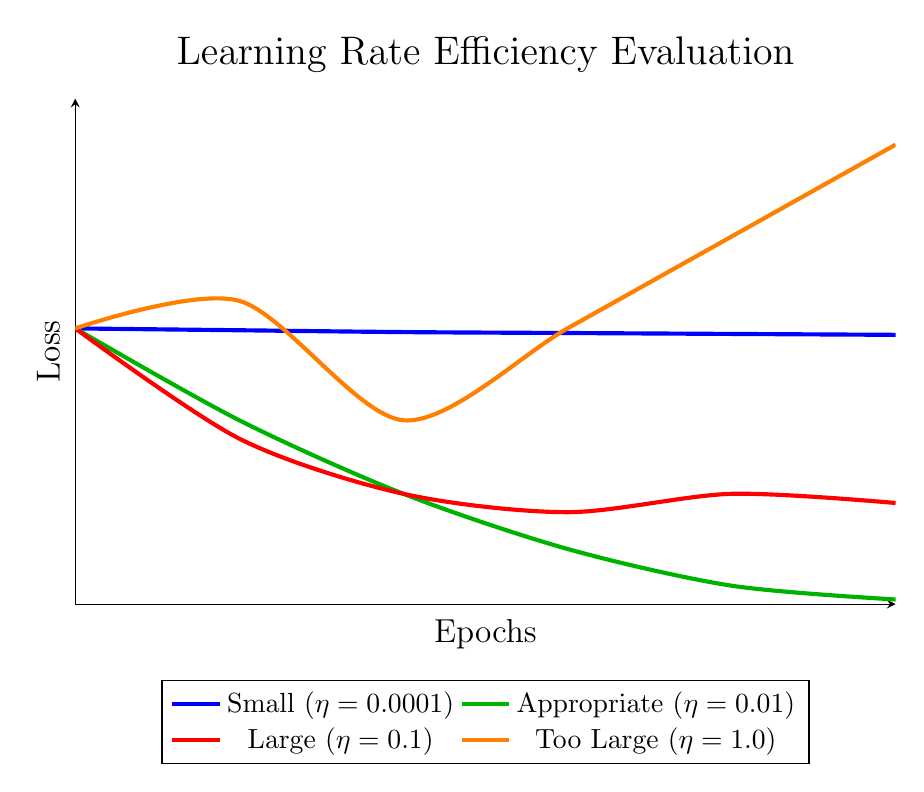
\begin{tikzpicture}
  \begin{axis}[
      width=12cm,
      height=8cm,
      xlabel={Epochs},
      ylabel={Loss},
      title={Learning Rate Efficiency Evaluation},
      tick label style={font=\large},
      label style={font=\large},
      title style={font=\Large},
      legend style={at={(0.5,-0.15)}, anchor=north, legend columns=2},
      axis lines=left,
      grid=none,
      ymin=0, ymax=55,
      xtick=\empty,
      ytick=\empty,
    ]
    
    % Small learning rate: very slow decrease (underfitting)
    \addplot[line width=1.5pt, smooth, color=blue, mark=none] coordinates {
      (0,30) (1,29.8) (2,29.6) (3,29.5) (4,29.4) (5,29.3)
    };
    \addlegendentry{Small ($\eta=0.0001$)}
    
    % Appropriate learning rate: rapid and stable convergence (loss nearly 0)
    \addplot[line width=1.5pt, smooth, color=green!70!black, mark=none] coordinates {
      (0,30) (1,20) (2,12) (3,6) (4,2) (5,0.5)
    };
    \addlegendentry{Appropriate ($\eta=0.01$)}
    
    % Large learning rate: fast initial drop with slight oscillation
    \addplot[line width=1.5pt, smooth, color=red, mark=none] coordinates {
      (0,30) (1,18) (2,12) (3,10) (4,12) (5,11)
    };
    \addlegendentry{Large ($\eta=0.1$)}
    
    % Too large learning rate: rises a little, then drops, then rises toward the end
    \addplot[line width=1.5pt, smooth, color=orange, mark=none] coordinates {
      (0,30) (1,33) (2,20) (3,30) (4,40) (5,50)
    };
    \addlegendentry{Too Large ($\eta=1.0$)}
    
  \end{axis}
\end{tikzpicture}

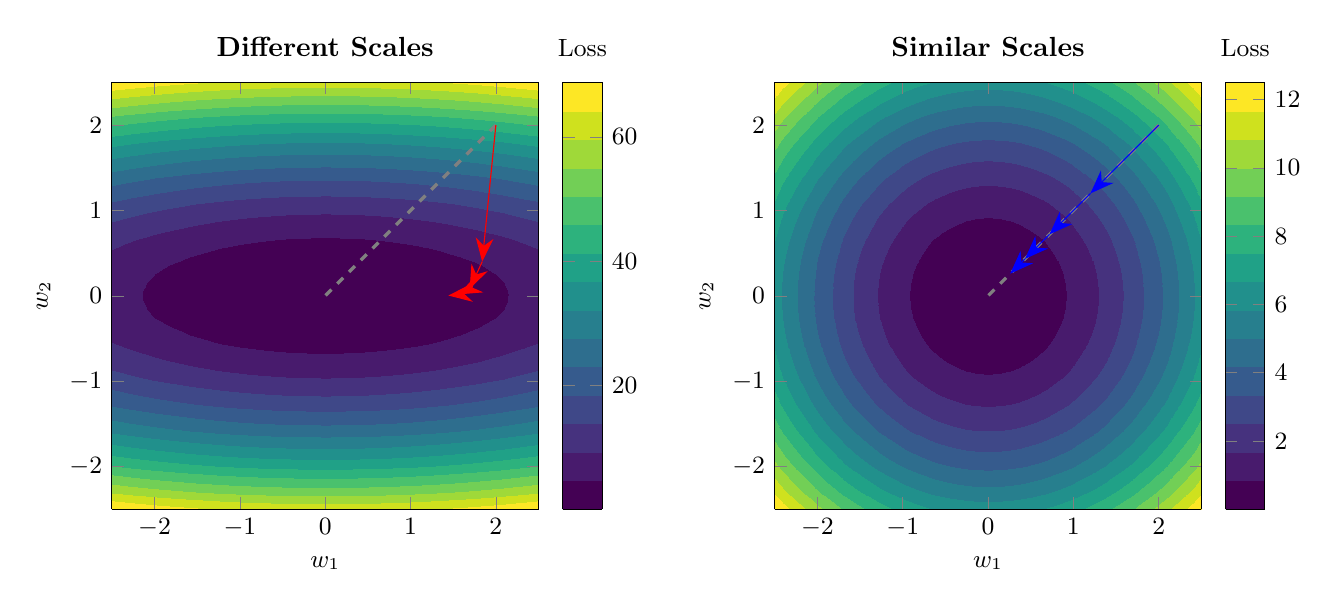
\begin{tikzpicture}[>=Stealth, font=\small]
  % DIFFERENT SCALES: Elliptical contours for f(w1,w2)= w1^2 + 10w2^2
  \begin{axis}[
      name=different,
      title={Different Scales},
      xlabel={$w_1$}, ylabel={$w_2$},
      axis equal,
      width=7cm, height=7cm,
      domain=-2.5:2.5,
      y domain=-2.5:2.5,
      samples=50,
      clip=false,
      view={0}{90},
      title style={font=\bfseries},
      colormap/viridis,
      colorbar,
      colorbar style={title=Loss},
    ]
    % Filled contour for f(w1,w2)= w1^2+10w2^2.
    \addplot3[
      contour filled={number=15},
      samples=50,
      domain=-2.5:2.5,
      y domain=-2.5:2.5,
    ] {x^2 + 10*y^2};
    
    % Global minimum direction: dashed gray line from (2,2) to (0,0)
    \addplot[
      dashed, gray, very thick,
      domain=0:1,
    ] ({2-2*x}, {2-2*x});
    
    % Gradient descent path (red arrows)
    % Iterations computed with learning rate α=0.04 starting at (2,2):
    %   (2,2) -> (1.84,0.4) -> (1.6928,0.08) -> (1.5574,0.016) -> (1.443,0.0032)
    \draw[red, -{Stealth[length=3mm]}] (axis cs:2,2) -- (axis cs:1.84,0.4);
    \draw[red, -{Stealth[length=3mm]}] (axis cs:1.84,0.4) -- (axis cs:1.6928,0.08);
    \draw[red, -{Stealth[length=3mm]}] (axis cs:1.6928,0.08) -- (axis cs:1.5574,0.016);
    \draw[red, -{Stealth[length=3mm]}] (axis cs:1.5574,0.016) -- (axis cs:1.443,0.0032);
  \end{axis}
  
  % SIMILAR SCALES: Circular contours for f(w1,w2)= w1^2 + w2^2
  \begin{axis}[
      at={(different.east)}, anchor=west, xshift=3cm,
      title={Similar Scales},
      xlabel={$w_1$}, ylabel={$w_2$},
      axis equal,
      width=7cm, height=7cm,
      domain=-2.5:2.5,
      y domain=-2.5:2.5,
      samples=50,
      clip=false,
      view={0}{90},
      title style={font=\bfseries},
      colormap/viridis,
      colorbar,
      colorbar style={title=Loss},
    ]
    % Filled contour for f(w1,w2)= w1^2+w2^2.
    \addplot3[
      contour filled={number=15},
      samples=50,
      domain=-2.5:2.5,
      y domain=-2.5:2.5,
    ] {x^2 + y^2};
    
    % Global minimum direction: dashed gray line from (2,2) to (0,0)
    \addplot[
      dashed, gray, very thick,
      domain=0:1,
    ] ({2-2*x}, {2-2*x});
    
    % Gradient descent path (blue arrows)
    % Iterations computed with learning rate α=0.2 starting at (2,2):
    %   (2,2) -> (1.2,1.2) -> (0.72,0.72) -> (0.432,0.432) -> (0.2592,0.2592)
    \draw[blue, -{Stealth[length=3mm]}] (axis cs:2,2) -- (axis cs:1.2,1.2);
    \draw[blue, -{Stealth[length=3mm]}] (axis cs:1.2,1.2) -- (axis cs:0.72,0.72);
    \draw[blue, -{Stealth[length=3mm]}] (axis cs:0.72,0.72) -- (axis cs:0.432,0.432);
    \draw[blue, -{Stealth[length=3mm]}] (axis cs:0.432,0.432) -- (axis cs:0.2592,0.2592);
  \end{axis}
\end{tikzpicture}

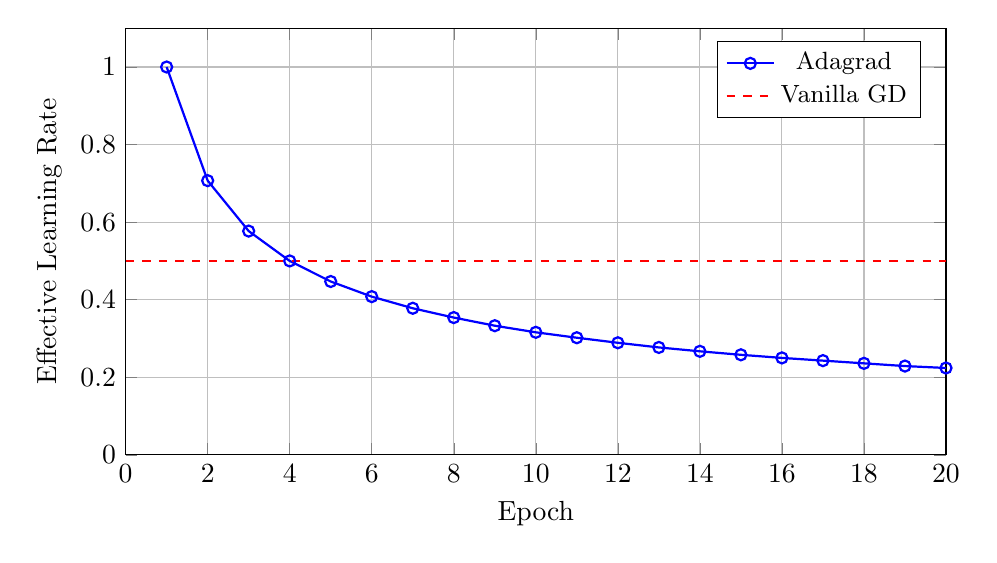
\begin{tikzpicture}
    \begin{axis}[
        width=12cm,
        height=7cm,
        xlabel={Epoch},
        ylabel={Effective Learning Rate},
        xmin=0, xmax=20,
        ymin=0, ymax=1.1,
        grid=major,
        legend pos=north east,
        legend style={font=\small}
    ]

    % Simulated effective learning rate (Adagrad)
    \addplot[color=blue, thick,mark=o] coordinates {
        (1,1)(2,0.707)(3,0.577)(4,0.5)(5,0.447)(6,0.408)(7,0.378)(8,0.354)(9,0.333)(10,0.316)(11,0.302)(12,0.289)(13,0.277)(14,0.267)(15,0.258)(16,0.25)(17,0.243)(18,0.236)(19,0.229)(20,0.224)
    };

    % Constant learning rate
    \addplot[dashed, red, thick] coordinates {
        (0,0.5)(20,0.5)
    };

    \legend{Adagrad, Vanilla GD}
    \end{axis}
\end{tikzpicture}
\end{document}

